% Welche Datenbank wurde verwendet und warum,...
\subsection{Anforderungen}
% TODO
Es wird eine moderne Plattform entwickelt, auf der sich Nutzer ähnlich Social Media Profile anderer Nutzer anschauen und miteinander Chats führen. Nutzer sollen in Echtzeit miteinander schreiben können und nahezu keine Wartezeit in Kauf nehmen müssen, um sich andere Profile anzeigen zu lassen. Die Datenbank muss nahezu immer erreichbar sein, da unsere Webseite ohne Datenbankanbindung nur beschränkt nutzbar ist.
Datenbank soll so designed sein, dass sie für die Zukunft des Projektes weiterhin gut geeignet ist.


Im Folgenden betrachten wir die Ziele, welche unsere Datenbank erfüllen muss und vergleichen die NoSQL Datenbank MongoDB mit PostgreSQL, welche repräsentativ für SQL basierte ORDBMS steht.

Logging
Backups
Reporting Tools
Sharding

\subsection{Geschichte}

\subsection{Lese- und Schreibgeschwindigkeit}
Um eine möglichst gute Benutzerfahrung zu gewährleisten, wird versucht, die Wartezeit beim Laden der Webseite zu verringern. 
Eine Möglichkeit dafür ist eine optimistische Benutzeroberfläche. Bei dieser wird davon ausgegangen, dass der angefragte Schreibzugriff erfolgreich ist; dem Nutzer wird bereits visuell der Erfolgsfall angezeigt. Sollte der Schreibzugriff fehlschlagen,  wird der Status der Benutzeroberfläche zurückgesetzt und der Nutzer durch eine Fehlermeldung informiert. Im Gegensatz zu einer realistischen Benutzeroberfläche, welche sich erst aktualisiert, wenn die Datenbank antwortet und der Schreibzugriff genehmigt wurde, erhält der Benutzer sofort eine Rückmeldung und muss nicht auf eine Antwort unseres Servers warten.
Anders als Schreibanfragen, welche mit einer Bestätigung oder Ablehung der Anfrage antworten, fordern Leseanfragen Daten an. Wartezeiten bei Leseanfragen können daher nicht maskiert werden.
Um in einem späteren Entwicklungsschritt die Reduzierung der Wartezeiten durch eine optimistische Benutzeroberfläche zu ermöglichen, werden daher langsamere Schreibgeschwindigkeiten in Kauf genommen, wenn sich mit dieser Entscheidung die Lesegeschwindigkeit erhöht.

SQL-Datenbanken wie PostgreSQL liegen meist in einer Normalform vor, um das Aktualisieren und Einfügen von Daten zu beschleunigen und die Konsistenz und Integrität gemäß ACID zu wahren. Neben diesen Vorteilen entstehen jedoch Nachteile, die sich negativ auf die Lesegeschwindigkeit auswirken. Dadurch, dass Daten nicht dupliziert werden, müssen bei Abfragen oft mehrere Tabellen zusammengeführt werden, wodurch Abfragen komplexer werden und die Effizienz von Indexen abnimmt. Beides wirkt sich negativ auf die Lesegeschwindigkeit aus. Um die Lesegeschwindigkeit zu erhöhen kann Denormalisierung verwendet werden, dies benötigt jedoch eine umfassende Umstrukturierung der bestehenden Daten, kann zu Anomalien in Datensätzen führen und benötigt weitere Schritte, um die Veränderung von Daten auf andere Tabellen zu übertragen. Wir halten dies für einen hohen Aufwand, der mit Risiko und hohen Kosten verbunden ist. 

MongoDB speichert Dokumente im JSON-Format und ermöglicht es, mehrere Werte für einen Schlüssel in Form eines Arrays zu hinterlegen. Auch ist es möglich, Dokumente in andere Dokumente einzubetten. Dies beschleunigt Leseabfragen, da die angeforderten Daten meist bereits in einem Dokument vorliegen, allerdings verringert sich die Schreibgeschwindigkeit, da Daten meist redundant in mehreren eingebetteten Dokumenten vorliegen und bei einer Änderung an mehreren Stellen überschrieben werden müssen. Anders als PostgreSQL ist MongoDB auf Grundlage dieser Art der Denormalisierung entworfen und ändert bei einem Schreibzugriff automatisch alle Instanzen des gleichen Dokumentes als Teil einer atomaren (Alles-oder-Nichts-)Transaktion. Auch Multi-Dokument-Transaktionen über verschiedene Shards und Replikatgruppen sind optional atomar. \cite{MG6}

\subsection{Flexible Datenstrukturen}
Im Rahmen des MVPs stehen die Projektanforderungen fest, allerdings soll im späteren Verlauf des Projektes auf die Wünsche der Nutzer geachtet werden und entsprechende Anpassungen an der Webseite getätigt werden. Datenstrukturen werden verworfen und angepasst, wenn sich diese nicht als nützlich erweisen. Speziell in der Anfangsphase eines Teilprojektes erlauben flexible Datenstrukturen eine Lösung zu entwickeln, welche mit wenig Zeitaufwand ein akzeptables Ergebnis liefert. Sollte sich das Teilprojekt als erfolgreich erweisen, kann in einem späteren Entwicklungsschritt die Lösung inkrementell perfektioniert werden. Eine Datenbank, die sich flexibel verändern lässt, ermöglicht es, schneller Anpassungen durchzuführen und verkürzt damit die Entwicklungszeit.

Tabellen in PostgreSQL können mit DDL-Befehlen wie ALTER TABLE verändert werden. Spalten können hinzugefügt, entfernt oder verändert werden, durch bestehende Constraints wird das Entfernen oder Ändern spezieller Spalten jedoch in einigen Fällen von der Datenbank verhindert, um die Integrität der Daten zu gewährleisten. Das Ändern des Datentyps einer Spalte ist in der Regel nur möglich, wenn die Datentypen zueinander kompatibel sind (zum Beispiel Integer zu Long) oder die Spalte für alle Datensätze leer ist. Erfahrungsgemäß bereitet das Ändern von bestehenden Spalten oft Probleme oder ist zumindest umständlich, vor allem, wenn andere Tabellen auf die zu ändernde Tabelle referenzieren.

MongoDB speichert Dokumente in Kollektionen, Dokumente der gleichen Kollektion müssen nicht die gleiche Struktur aufweisen, da das Dokument dessen Struktur nach JSON-Spezifikation (durch die Angabe der Schlüssel-Wert-Paare) selbst beinhaltet. Dementsprechend können Dokumente mit neuen, anderen oder fehlenden Attributen direkt zu bestehenden Kollektionen hinzugefügt werden können. Dies erlaubt es uns, bei der Weiterentwicklung von Kollektionen direkt die neuen Dokumente in bestehende Kollektionen einzufügen, ohne bestehende Dokumente verändern zu müssen, was Zeit spart und sich im Falle eines Fehlers einfach zurückrollen lässt. Es sollte Wert auf die Abwärtskompatibilität gesetzt werden, damit bestehende Schnittstellen ohne Veränderung weiter funktionieren.

% MongoDB bietet mehr Optionen der Flexibilität und eignet sich daher in diesem Punkt für das Projekt besser.

\subsection{Hochverfügbarkeit}
Für den Anmeldevorgang, die Registrierung und alle Seiten unserer Plattform, die einen angemeldeten Nutzer voraussetzen, ist eine Datenbankanbindung zwingend erforderlich. Diese Teile machen den Großteil der Webseite aus, jede Minute, in der die Datenbank ausfällt, fällt unser Service nahezu komplett aus. Es bietet sich eine Datenbank mit Hochverfügbarkeit an, um das Risiko eines Ausfalls unserer Plattform so weit wie möglich zu verringern.
Um die Erreichbarkeit der Datenbank zu gewährleisten, bietet es sich an, Replikatgruppen zu erstellen. Eine Replikatgruppe besteht aus mehreren Datenbankprozessen, auch Knoten genannt, welche den gleichen Datensatz verwalten. Sollten durch Hardwarefehler einzelne Knoten ausfallen oder Softwarefehler Knoten dazu zwingen, neu gestartet zu werden, ist die Datenbank, wenn auch mit verringerter Leistung, weiterhin erreichbar. Die dadurch erreichte Fehlertoleranz schafft Sicherheit und verringert die Chance, dass die Datenbank komplett ausfällt drastisch. Meist hat nur ein Prozess der Replikatgruppe Schreibrechte, um die Konsistenz bei gleichzeitigen Schreibzugriffen zu wahren. Neben diesem Primärknoten existieren oft mehrere Sekundärknoten, welche die Schreibvorgänge des Primärknotens kopieren und für Lesezugriffe zur Verfügung stehen. Es existieren andere Architekturen mit mehreren Primärknoten, die gleichzeitige Schreibzugriffe erlauben und besondere Herausforderungen bei der Datenkonsistenz stellen, diese werden hier jedoch nicht betrachtet.

PostgreSQL bietet verschiedene Lösungsansätze. Bei synchronen Lösungen muss ein Schreibauftrag von allen Knoten durchgeführt sein, um als bestätigt zu gelten. Asynchrone Lösungen erlauben einen Puffer zwischen dem Bestätigen eines Schreibauftrags und dessen Kopie auf andere Knoten, wodurch das Wechseln zu einem Backupknoten zu Datenverlust führen kann und Sekundärknoten bei Lesezugriffen ein leicht veraltertes Ergebnis liefern können. Dafür gewinnt eine asynchrone Lösung an Performanz, da sich die Wartezeit stark verringert. Um die Knoten auf dem gleichen Stand zu halten und im Fall eines Ausfalls Daten wiederherstellen zu können, wird ein \textit{Write-Ahead Log} (WAL) angelegt, welcher unmittelbar nach jedem Commit die Transaktion in einen Transaktionslog schreibt. Dieser wird dann von anderen Knoten ausgelesen und die Transaktion wird kopiert. \cite{PG1} Sollte der Primärknoten ausfallen, muss dies detektiert werden und ein Sekundärknoten mit so wenig Verzögerung wie möglich als neuer Primärknoten ausgewählt werden. Leider bietet PostgreSQL keine automatische Ausfallsicherung, es muss daher eine Drittanbietersoftware verwendet werden oder ein eigener Skript geschrieben werden. Um die Belastung der einzelnen Knoten möglichst gleich zu halten, sollte ein Prozess zur Lastverteilung existieren. Unseren Recherchen nach bietet PostgreSQL selbst keine native Lastverteilung, meist wird die kostenlose Open-Source Software HAProxy (High Availability Proxy) verwendet.

Knoten in MongoDBs Replikatgruppen teilen sich gegenseitig durch Ping-Befehle ihren \enquote{Herzschlag} mit, um zu ermitteln, ob ein Knoten ausgefallen ist. Sollte der Primärknoten \enquote{sterben}, wählen die \enquote{überlebenden} Knoten in einer Abstimmung den nächsten Primärknoten, welcher die Schreibaufträge des vorigen Primärknotens übernimmt. Der Prozess einer Wahl sollte in der Regel nicht länger als 12 Sekunden dauern und passiert vollautomatisch, der Endbenutzer sollte bis auf gegebenenfalls eine kurze Wartezeit vom Wechsel nichts erfahren. Knoten mit mehr Leistung kann eine höhere Priorität zugewiesen werden, um diesen als präferierten Primärknoten zu definieren. Auch eignet es sich, Knoten in anderen Regionen für die Rolle des Primärknoten als unwählbar zu definieren, da sich die Latenz ansonsten drastisch erhöhen würde. Ein Replikset kann aus maximimal 50 Knoten bestehen, wovon bis zu 7 zum Primärknoten wählbar sind. \cite{MG1} \cite{MG2} Diese Zahl wirkt groß genug, um einen gleichzeitigen Ausfall aller Knoten aus technischer Sicht nahezu unmöglich zu gestalten, sollten sich die Knoten zusätzlich auf verschiedenen physischen Geräten befinden.
In seltenen Fällen kann es vorkommen, dass der Primärknoten ausfällt und vor seinem Ausfall Schreibaufträge bestätigt, diese aber nicht an die Standbyknoten weiterleiten kann. Wenn der frühere Primärknoten der Replikatgruppe wieder beitritt, in diesem Fall als Sekundärknoten, unterscheidet sich dessen Schreibhistorie von der anderer Knoten. Die Historie des früheren Primärknoten wird zurückgerollt und die bestätigten Schreibaufträge sind verloren. MongoDB versucht durch verschiedene Techniken, Rollbacks zu vermeiden und erlaubt es unter Verlust von Effizienz, mit Schreibbestätigungen erst zu antworten, wenn der Großteil der Replikatgruppe diese bestätigt hat. Sollte es trotzdem zu einem Rollback kommen, müssen einzelne Schreibaufträge oft manuell nach bestem Gewissen der Datenbankexperten wiederholt werden. \cite{MG3} Leseanfragen werden per Standardkonfiguration an den Primärknoten gestellt, um möglichst aktuelle Daten liefern zu können. Diese Präferenz lässt sich ändern, um den Primärknoten zu entlasten, auf speziell eingerichtete Knoten mit optimisierten Indexen zugreifen zu können, die Latenz zu verringern oder beim Ausfall des Primärknotens weiterhin Lesezugriffe zu ermöglichen.

MongoDB überzeugt im Punkt der Hochverfügbarkeit gegenüber PostgreSQL. Um PostgreSQL hochverfügbar zu machen, sind einige Anpassungen und Expertenwissen oder Drittanbietersoftware nötig. MongoDB scheint von der Architektur auf Hochverfügbarkeit ausgerichtet zu sein und liefert Funktionen für eine automatische Ausfallsicherung, welche das System nach kurzer Zeit ohne manuelle Eingriffe wieder voll funktionstüchtig machen. Wir glauben, dass mit MongoDB eine Datenbank eingerichtet werden kann, die mit wenig Aufwand stabil für sehr geringe Ausfallraten sorgen kann.

\subsection{Skalierbarkeit}
% https://www.grin.com/document/286400
% https://db-engines.com/de/article/Sharding
Mit jeden neuen Nutzer unserer Plattform steigt die Diversität und somit die Chance, dass sich zwei Nutzer finden, welche zusammen passen und sich anfreunden. Je mehr Teilnehmer unserem Netzwerk angehören, desto höher ist die Anzahl der potenziellen Kommunikationspartner und somit der Nutzen und Wert der Plattform. Wir sprechen von einem positiven direkten Netzwerkeffekt. Je größer der Nutzer der Plattform, desto eher werden Webseitenbesucher weiteren potenziellen Besuchern von der Webseite erzählen, wodurch die Plattform weiter wächst und ihren Nutzen weiter ausbaut. Dies kann zu exponenziellem Wachstum führen. Desweiteren können große Persönlichkeiten der sozialen Medien (\enquote{Influencer}) mit einer einzigen Bemerkung tausende Personen davon überzeugen, einen Blick auf unsere Webseite zu werfen.
Eine kurzfristige, rapide Vergrößerung der Nutzerbasis und exponenzielles Wachstum stellen Datenbanken vor eine Herausforderung, die sich mit Skalierung lösen lässt. Auch sollen die Kapazitäten der Datenbank flexibel verringert werden können, um in Zeiten, in der die Datenbank nicht ausgelastet ist, finanzielle Mittel zu sparen. Zur Skalierung wird eine Kombination aus vertikaler Skalierung (Leistungsfähigere Hardware) und horizontaler Skalierung (mehr Geräte nebeneinander betrieben) gewählt. Vertikale Skalierung stößt auf Limitierungen, da der Preis von leistungsfähiger Hardware exponenziell Skaliert. Weitere Skalierung ist dann nicht mehr rentabel. Bei horizontaler Skalierung müssen die einzelnen Knoten miteinander kommunizieren, die für die Kommunikation benötigten Ressourcen steigen mit jedem weiteren Knoten. Aus diesem Grund limitieren manche Datenbanken die Maximalanzahl an Knoten in einer Replikatgruppe. \cite{MG6} Desweiteren kann Datenbanksharding, eine Art der Datenbankpartitionierung betrieben werden, bei dem eine Datenbank in mehrere Splitter bzw. Scherben aufgeteilt wird, welche jeweils einen Teil der Daten verwalten. Durch diese Verfahren können Datenmengen verarbeitet werden, welche die Kapazität einer einzelnen Replikatgruppe übertreffen würde.

\subsection{Vertikale Skalierung}
Nahezu jede Datenbank lässt sich mit leistungsfähiger Hardware vertikal Skalieren, so auch PostgreSQL und MongoDB. Zwischen den beiden Datenbanken gibt es dahingehend keine nennenswerten Unterschiede
Sowohl MongoDB als auch PostgreSQL lassen sich vertikal skalieren, beim Vergleich wird daher die horizontale Skalierung und Sharding verglichen.

%TODO
\subsubsection{Horizontale Skalierung}
PostgreSQL

MongoDB

\subsubsection{Sharding}
Sharding stellt PostgreSQL vor eine Herausforderung, da komplexe JOIN-Anweisungen meist Daten von verschiedenen Shards erfragen, welche untereinander kommunizieren müssen. Diese Abfragen benötigen unverhältnismäßig viele Ressourcen und machen Performanzgewinne des Shardings zunichte. Es ist daher darauf zu achten, Shards so zu konzipieren, dass Anfragen dieser Art so solten wie möglich vorkommen.

MongoDB setzt auf Dokumente, welche in den meisten Fällen nicht auf Referenzen zu anderen Dokumenten angewiesen sind. JOIN-artige Anweisungen werden eher selten verwendet, Dokumente sind meist flacher als die Pendants der SQL-Tabellen. Dadurch entstehen weniger komplexe Abfragen, in welchen Dokumente verschiedener Shards kombiniert werden müssen, die Datenbank wird weniger beansprucht. Sharding in MongoDB ist mit niedrigen Kosten verbunden und benötigt selten eine exakt konzipierte Struktur; es ist verhältnismäßig einfach, mit Sharding eine MongoDB Datenbank zu skalieren.

%TODO delete this
\subsection{Skalierbarkeit}
Webseiten wie unsere können "über Nacht" zum Erfolg werden, es reicht ein großer Influencer, welcher seinen Followern von der Webseite berichtet und auf einen Schlag erreichen wir Nutzerzahlen, bei denen unsere Rechenleistung auf Grenzen stößt. Die Datenbank unserer Wahl sollte sich vor allem schnell, ohne viel Programmieraufwand, skalieren lassen, um die Zeit, in denen unsere Plattform ausgelastet ist, möglichst gering zu halten.
\subsubsection{Skalierbarkeit}
Sowohl PostgreSQL als auch MongoDB lassen sich vertikal skalieren - mit mehr Ressourcen läuft die Datenbank schneller. Bei horizontaler Skalierung verfolgen die beiden Datenbanken verschiedene Ansätze.
\paragraph{PostgreSQL} nutzt ein Master-Slave-System bzw. Primary-Standby-System mit Lastverteilung.\cite{PG6} Die Standby-Knoten sind Kopien des Primärknotens und können Lesezugriffe verarbeiten. Schreibzugriffe werden nur vom Primärknoten angenommen. Sollte der Primärknoten versagen, bietet PostgreSQL keine automatische Lösung dieses Problems, ohne Drittsoftware muss manuell ein neuer Primärknoten gewählt werden. Es gibt nur einen Primärknoten, für Multi-Master-Systeme wird Drittsoftware benötigt. Selbst mit synchronen Repliken dauert es einen Moment, bis die Standby-Knoten die Aktualisierungen der Datenbank übernommen haben, dies kann dazu führen, dass Abfragen mit veralteten Datensätzen beantwortet werden.\cite{PG8} Consistency nach CAP-Theorem ist für PostgreSQLs Master-Slave-Systeme somit nicht mehr einhundertprozentig gegeben.
Durch Sharding lässt sich die Datenbank in einzelne Knoten aufteilen, die jeweils nur einen Teil der Daten beinhalten. Dies erlaubt es, die Last und benötigte Speicherkapazität pro Knoten weiter zu verringern. Es ist möglich, mehrere Shards vom gleichen Knoten verwalten zu lassen; dies erleichtert die Skalierung, da die Anzahl der Shards flexibel an die technischen Ressourcen des verwaltenden Knoten angepasst werden kann.
\paragraph{MongoDB}
benutzt Replik-Sets, welche ähnlich wie das vorgestellte Master-Slave-System von PostgreSQL funktionieren. Der Primärknoten ist der einzige Knoten mit Schreibzugriff und repliziert die Änderungen auf die Sekundärknoten. Alleridngs hat MongoDB ein automatisches System, welches einen Ausfall des Primärknotens abfängt. Alle Knoten teilen den anderen Knoten ihren \enquote{Herzschlag} mit, in dem sie sich gegenseitig anpingen. Sollte der Herzschlag des Primärknotens ausfallen, wählen die Sekundärknoten unter ihnen einen neuen Primärknoten aus, welcher dann die Aufgaben des früheren Primärknotens übernimmt. Es ist möglich, Knoten mit mehr Rechenleistung eine höhere Priorität zuzuweisen, um die Wahrscheinlichkeit zu erhöhen, dass dieser Knoten der nächste Primärknoten wird. Auch ist es möglich, zu verhindern, dass spezielle Knoten Primärknoten werden, dies ist ratsam für Knoten, die schlechtere Hardware besitzen oder eine höhere Latenz aufweisen, weil sie beispielsweise in einer entfernten Region stehen. Den Knoten können zudem verschiedene Rollen zugewiesen werden, versteckte Knoten können für Datenbankauswertungen verwendet werden, während verzögerte Knoten einen historischen Schnappschuss der Datenbank speichern und Aktualisierungen der Datenbank mit einer Verzögerung ausführen und somit als Backup dienen können. \cite{MG10}\cite{MG11}\cite{MG12}\cite{MG13} MongoDB erlaubt zudem Systeme mit mehreren Primärknoten, in den meisten Fällen sind Optionen wie Sharding jedoch besser geeignet. \cite{MG14}
Shards wiederum können als eigene Replica-Sets eingesetzt werden. Dies erlaubt es, für verschiedene Regionen eigene Shards der Datenbank einzurichten, welche dann wiederum in einem eigenen Replica-Set gesteuert werden.



\subsection{}

\subsubsection{Dateiformat}
MongoDB speichert Daten im \glqq binary JSON\grqq -Format. JSON, die \glqq JavaScript Object Notation \grqq, ist \enquote{ein schlankes Datenaustauschformat, welches für Menschen einfach zu lesen und für Maschinen einfach zu parsen [] ist} \cite{JSON1}. JSON als semistrukturiertes Dateiformat eignet sich gut für Schnittstellendaten. Zudem wird im gewählten MERN-Techstack ausschließlich JavaScript verwendet - das JavaScript native Dateiformat JSON ist daher ohne Umwandlungen direkt verwendbar und der Umgang für unsere Entwickler bereits bekannt. Dies verringert die Gefahr möglicher Komplikationen und spart Lern- und Programmieraufwand.

\subsubsection{Fazit}
Wir haben nach einer Datenbank gesucht, welche bei Leseanfragen schnell antwortet, schnelle Änderungen der Datenstrukturen zulässt, eine hohe Erreichbarkeit aufweist und sich schnell und einfach skalieren lässt. Dafür nehmen wir langsamere Schreibanfragen und Inkonsistenz bei Leseanfragen in Kauf. Wir konnten zeigen, dass sowohl PostgreSQL als auch MongoDB ausgereifte Lösungen sind, sich MongoDB als Gesamtpaket für unsere speziellen Anforderungen besser eignet.
%Begründen

\subsubsection{PostgreSQL}
Michael Stonebreaker veröffentlichte 1974 in Berkeley unter BSD-Lizenz das RDBMS INGRES. Jahre später führte er das Projekt als Postgres (Post INGRES) weiter und fügte einen objektorientierten Ansatz hinzu. \cite{PG1} Im Laufe der Jahre wurde PostgreSQL fortlaufend weiterentwickelt und hat viele neue Funktionen dazuerhalten.
PostgreSQL beschreibt sich selbst als \enquote{das fortschrittlichste, quelloffene, relationale Datenbankmanagementsystem und habe sich in über 30 Jahren aktiver Entwicklung einen guten Ruf für Zuverlässlichkeit, Funktionsrobusheit und Leistung verdient}. \cite{PG2} PostgreSQL soll auch in Zukunft unter einer quelloffenen Lizenz stehen, welche die kommerzielle Nutzung erlaubt. \cite{PG3}
PostgreSQL wurde exemplarisch als Option eines SQL-Systems verwendet, da der Funktionsumfang vergleichbar mit anderen beliebten SQL-Systemen ist. \cite{PG4}

\subsubsection{MongoDB}
Die 2007 neu gegründete Firma 10Gen, mittlerweile bekannt als MongoDB Inc., benötigte eine Datenbank, welche den Anforderungen ihrer quelloffenen Plattform-as-a-Service Cloud-Architektur gerecht werden würde. Das Team suchte nach einer Datenbank, die elastisch, skalierbar, einfach zu verwalten und für Entwickler und Anwender einfach zu benutzen ist. Unzufrieden mit den zu der Zeit auf dem Markt verfügbaren Datenbanksystemen wurde MongoDB, eine dokumentbasierte Datenbank entwickelt. Als das Team das Potenzial der Datenbank realisierte, wurde die Idee der Cloud-Plattform eingestellt und die Entwicklung von MongoDB gefördert.\cite{MG1}
Laut eigenen Aussagen ist \enquote{MongoDB [] eine universelle, dokumentbasierte, verteilte Datenbank für die moderne Anwendungsentwicklung und die Cloud, die in puncto Produktivität höchsten Ansprüchen gerecht wird}. \cite{MG2} 

%TODO delete this - compare advantages/disadvantages instead
\subsubsection{MongoDB und PostgreSQL im Vergleich}

\begin{center}
    \begin{tabularx}{\linewidth}{ |X|X|X| } 
     \hline
     Kriterien & PostgreSQL & MongoDB  \\ 
     \hline
     Datenbanktyp & SQL, Objektrelational & NoSQL, Dokumentbasiert \\
     Ranking nach DB-Engines \cite{DB1} & 577,50 Punkte, viertbeliebteste Datenbank, viertbeliebteste relationale Datenbank & 496,50 Punkte, fünftbeliebteste Datenbank, beliebteste nicht-relationale Datenbank \cite{DB2} \\
     Architektur & Monolithisch & Dezentralisiert \\
     Erscheinungsjahr & 1989 & 2009 \\
     Datenschema & Ja & Selbstbeschreibende Dokumente\\
     Referenzierung & Referenzierung per ID, erlaubt Foreign Keys & Referenzierung per ID oder eingebettetes Sub-Dokument \\
     Datenstruktur & Tabellen bestehen aus Zeilen und Spalten & Kollektionen bestehen aus Dokumenten. Dokumente haben Felder. Dokumente der gleichen Kollektion müssen nicht die selben Felder besitzen. \\
     Typisierung & Erlaubt verschiedene Datentypen und nutzerdefinierte Datentypen\cite{PG5} & Erlaubt verschiedene Datentypen nach BSON Spezifikation \cite{MG3}; ähnelt stark JSON \\
     Horizontale Skalierung & Repliken nach Master-Slave-System \cite{PG6} & Sharding und Replica Sets als Teil der Infrastruktur \cite{MG4} \cite{MG5} \\
     Konsistenzmodell & ACID, optional eventuelle Konsistenz \cite{MG6} \cite{MG7} & ACID \\
     \hline
    \end{tabularx}
    \cite{DB3} \cite{DB4}
\end{center}

\subsubsection{ACID}
 MongoDB ist seit Erschaffung auf Dokumentebene ACID-Konform und ab den Versionen 4.0 (Juni 2018 \cite{MG8}) auf einem einzelnen Replik-Set bzw. ab Version 4.2 (August 2019 \cite{MG8}) zwischen mehreren Replik-Sets bei multi-Dokument-Transaktionen ACID-Konform. \cite{MG6} Dies erlaubt "Alles-oder-Nichts"-Transaktionen, bei denen es kritisch ist, dass entweder alle Teile oder kein Teil der Transaktion ausgeführt wird und löst damit Probleme, die historisch nur mit SQL-Datenbanken lösbar waren.

\subsubsection{Referenzierung und Denormalisierung}
PostgreSQL erlaubt, andere Tabellen mit Foreign Keys (FK) gemäß SQL-Standard zu referenzieren. Der Wert eines FK muss korrekt sein, sollte der angegebene FK in der referenzierten Tabelle nicht existieren, wird ein Fehler geworfen. Auch ist es möglich, entsprechende Regeln zu definieren, was passieren soll, wenn der referenzierte Datensatz beispielsweise gelöscht wird.
MongoDB ermöglicht auch, andere Dokumente per ID zu referenzieren, bietet jedoch keine direkte Option, zu definieren, was beim Löschen des referenzieren Datensatzes passieren soll. Es ist weiterhin möglich, Trigger beim Löschen des referenzierten Datensatzes feuern zu lassen, dies hat im Vergleich zum Foreign Key Constraint allerdings eine höhere Komplexität. Stattdessen setzt MongoDB darauf, alle relevanten Informationen soweit möglich in einem Dokument einzubetten.
%TODO Schaubilder erstellen 1-1 1-Many Many-Many

Eingebettete Dokumente erlauben schnelleren Lesezugriff, da sich alle relevanten Informationen in einem Dokument befinden und - anders als in SQL - nicht über mehrere Tabellen mit im Laufe des Produktlebenszyklus immer komplexeren JOIN-Anweisungen zusammengefasst werden müssen. Dies vereinfacht das Schreiben von Abfragen und erhöht die Geschwindigkeit von Leseabfragen. Als Nachteil wird dabei in Kauf genommen, dass Daten über verschiedene Dokumente dupliziert werden und Schreibzugriffe dadurch langsamer werden - schließlich müssen Daten in verschiedenen Dokumenten erstellt oder aktualisiert werden. 
Jedes Mal, wenn das Profil eines Nutzers in der Kontaktsuche angezeigt werden soll oder wenn die Freundesliste oder ein Chat geöffnet wird, muss das Profil dieses Nutzers abgefragt werden. Das kann teilweise für hunderte Anfragen pro Profil am Tag sorgen und belastet entsprechend unsere Datenbank. Den Projektanforderungen nach ist außerdem wichtig, dass Nutzer schnell Profile angezeigt bekommen. Schreibanfragen, bei denen ein neues Profil erstellt wird oder ein Nutzer sein eigenes Profil aktualisiert, werden weitaus seltener vorkommen als Leseanfragen. Auch sind wir der Meinung, dass Nutzer eine längere Wartezeit bei Profilaktualisierungen eher hinnehmen, als bei Lesezugriffen zu warten.
Entsprechend sind wir der Meinung, dass für unser Projekt die Vorteile eingebetteter Dokumente dessen Nachteile überwiegen.



\begin{figure}[ht]
	\centering
    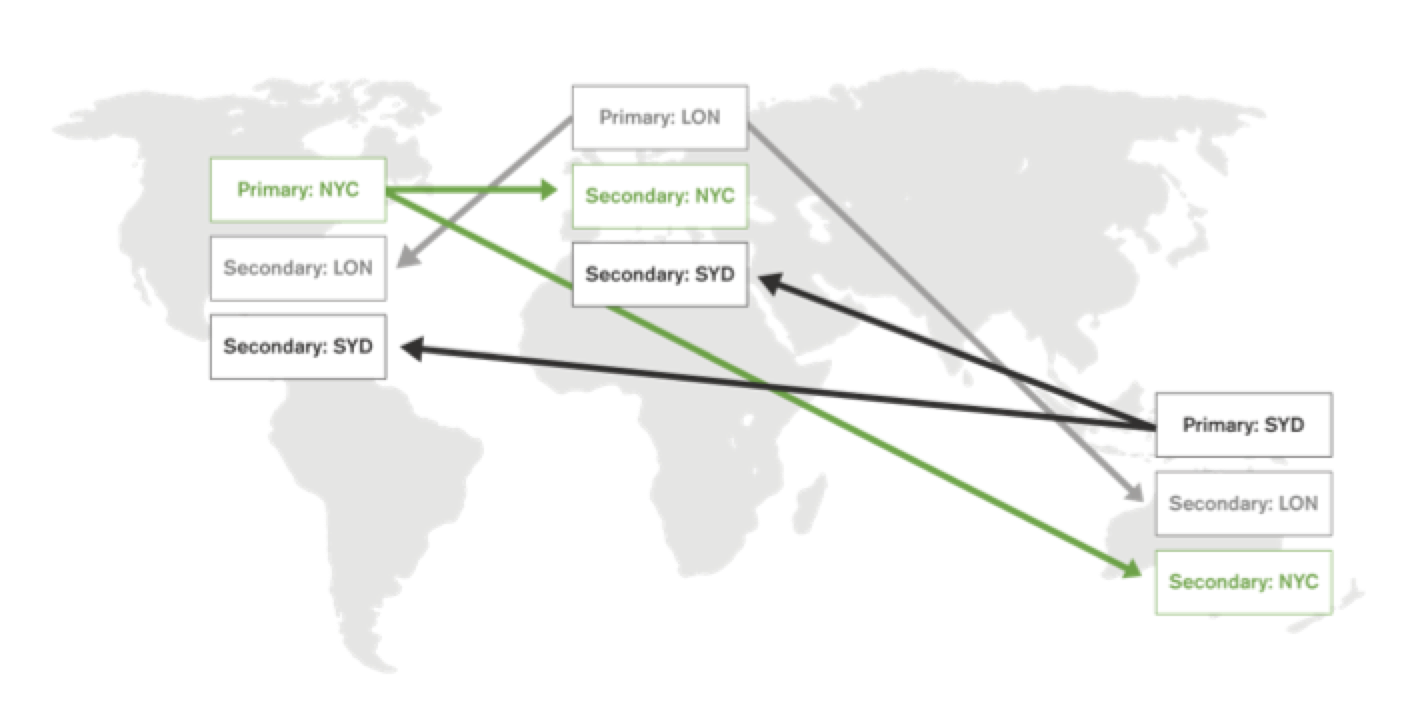
\includegraphics[width=\textwidth]{sources/MongoDB_sharded.png}\cite{MG14}
	\caption{Aktiv-Aktiv-Architektur mit Datenbank-Sharding}
	\label{fig1}
\end{figure}

Jedes Jahr fallen größere Mengen an Daten an. Durch diese Entwicklung ist die Möglichkeit, horizontal skalieren zu können, immer wichtiger geworden. Zur Anfangszeit von PostgreSQL hat es für die meisten Projekte gereicht, vertikal zu skalieren, erst über die Jahre wurden Techniken zur horizontalen Skalierung entwickelt. Für Techniken wie der automatischen Wahl eines neuen Primärknotens oder Multi-Master-Systemen benötigt es Drittsoftware. In MongoDB ist horizontale Skalierung seit jeher wichtige Priorität und ist als solches stark in die Datenbankinfrastruktur eingebettet. Wir sind der Meinung, dass die von MongoDB verwendeten Lösungen zur horizontalen Skalierung ausgereifter sind und gleichzeitig weniger fachliches Wissen benötigen und damit entsprechend schneller und einfacher durchführbar sind.



\subsection{Schemata}
Folgende Kollektionen wurden verwendet, um die Daten optimal zu verwalten.

\subsubsection{Nutzer}
\begin{center}
    \begin{tabularx}{\textwidth}{ |X|X|X| } 
     %\hline
     %Feld & Beschreibung & Beispiel \\ 
     %\hline
     % _id & Standardmäßige MongoId & \\
     % Benutzername & einzigartiger, öffentlicher Name & MaxMustermann \\ 
     % normalisierter Name & Name in Kleinbuchstaben. Wird verwendet, um die Einzigartigkeit von Namen zu gewährleisten & maxmustermann \\ 
     % Email & private eMail des Nutzers & mustermann@email.de \\
     % Rolle & Gibt an, ob der Nutzer autorisiert ist - Moderatoren und Administratorkonten haben mehr Rechte. Automatisch generiert & Nutzer \\ 
     % Geburtsdatum & privates Geburtsdatum des Nutzers & 01.01.2000 \\ 
     % Alter & Alter des Nutzers. Wird automatisch mit Geburtsdatum berechnet & 21 \\ 
     % Sprachen & Array von Sprachen, die der Nutzer sprechen kann & [de, en] \\
     % Geschlecht & gesellschaftliches Geschlecht des Nutzers. & Männlich \\ 
     % Spielposition & Bis zu 2 Lieblingspositionen des Spielers in League of Legends & [Mid, Jungle] \\ 
     % Freitext & kurzer Text, in dem der Nutzer sich beschreiben kann. & Ich bin ein toller Nutzer! \\
     % Avatar & URI [GLOSSAR!] vom Avatarbild des Nutzers & https://<s3-name>.s3.eu-central-1.amazonaws.com/avatars/<UUID>.jpg \\ 
     % Freunde & Array von allen Freunden des Nutzers. Beinhaltet die NutzerID und die ChatID & [[_id1, NutzerID1, ChatID1], [_id2, NutzerID2, ChatID2]]\\ 
     % Geblockt & Array von NutzerIDs der Nutzer, die geblockt wurden & [NutzerID3, NutzerID4] \\ 
     %\hline
    \end{tabularx}
\end{center}

Wenn ein Nutzer einen Account erstellt, gibt dieser dessen eMail, den gewünschten Benutzernamen und das gewünschte Passwort an. Durch Indexe wird die Einzigartigkeit von eMail und Benutzername geprüft, das Passwort wird aus Sicherheitsgründen in einer separaten Kollektion gespeichert. Nach der Kontoerstellung kann der Nutzer das Geburtsdatum, die gesprochenen Sprachen, das Geschlecht, die Spielposition und einen Freitext angeben und ein Bild hochladen, welches als Avatarbild dient. Felder wie der normalisierte Name, das Alter und die Rolle werden automatisch generiert. Im Laufe der Nutzung unserer Plattform wird der Nutzer andere Spieler als Freunde hinzufügen - diese werden in einer Freundesliste gespeichert. Auch steht es dem Nutzer frei, Andere zu blockieren - in diesem Fall wird die NutzerID des Blockierten auf die Blockliste hinzugefügt.
Privatsphäre und damit die Sicherheit der eigenen Daten ist uns wichtig. Wir wollen daher die Anzahl an Daten, die ein Nutzer von sich preisgeben müssen, so gering wie möglich halten. Die Email-Adresse, das Geburtsdatum und Freundes- und Blockliste sind für andere Nutzer nicht einsehbar, bis auf den Benutzernamen muss eine Person keine Daten öffentlich angeben.

\subsubsection{Sprache}
Damit Nutzer ihre Sprache wählen können, bieten wir die Wahl zwischen 187 Sprachen nach ISO 639-1 Norm an.\cite{ISO639-1} 

\begin{center}
    \begin{tabular}{ |c|c|c| }
        \hline
        Feld & Beschreibung & Beispiel \\
        \hline
        id & Alpha-2 Code der Sprache & en, de, fr \\
        name & Englische Schreibweise der Sprache & English, German, French \\
        nativer Name & native Schreibweise der Sprache & English, Deutsch, français \\
        \hline
    \end{tabular}
\end{center}
Normale Objekt-IDs von MongoDB enthalten einen Zeitstempel und einen inkrementellen Zähler.\cite{MG15} Diese Daten halten wir bei Sprachen, also öffentlichen Stammdaten, die sich über einen langen Zeitraum nicht verändern werden, nicht sinnvoll. Stattdessen haben wir den Alpha-2-Code der Sprache als ID gewählt, der auf die Sprache schließen lässt. Nutzerdokumente referenzieren die Sprache per ID, dies erlaubt es uns, direkt im Nutzerdokument anhand der Sprach-ID zu erkennen, welche Sprachen der Nutzer spricht.
Sprachen können sowohl anhand der englischen Schreibweise als auch der nativen Schreibweise gefunden werden. Dies erleichtert Nutzern auch nicht-englischsprachigen Nutzern, ihre Sprache auswählen zu können.

\subsubsection{Passwort}
\begin{center}
    \begin{tabular}{ |c|c| }
        \hline
        Feld & Beschreibung  \\
        \hline
        id & Standardmäßige MongoId \\
        password & Bcrypt Hash bestehend aus Versionsnummer, Komplexität, Salt und Hash \\
        NutzerID & MongoId des zugehörigen Nutzers \\
        \hline
    \end{tabular}
    \cite{DB3} \cite{DB4}
\end{center}

Das Passwort wird nicht im Nutzerdokument gespeichert. Würde das Passwort im Nutzerdokument gespeichert werden, könnte es schon durch kleine Programmierfehler dazu kommen, dass normale Nutzer das gehashte Passwort anderer Nutzer ermitteln könnten. Um dieses Sicherheitsproblem direkt zu eliminieren, wird daher für jedes Passwort ein eigenes, vom Nutzerdokument isoliertes Dokument verwendet.
Das Passwort wird durch bcrypt, einem Blowfish-basiertem Hashalgorithmus, auf der Datenbank als Hash mit Salt gespeichert. Die Komplexität des Hashes ist durch uns wählbar. Bei der Wahl der Komplexität ist die Sicherheit gegen Rechengeschwindigkeit abzuwägen; eine höhere Komplexität erhöht die benötigte Zeit pro Versuch eines Angreifers, das Passwort zu knacken, erhöht gleichzeitig aber auch die Zeit, die unser Server benötigt, um ein neues Passwort zu generieren oder den Anmeldeversuch eines ehrlichen Nutzers zu bestätigen. Eine zu hohe Komplexität kann daher unseren Server stark verlangsamen und macht Angriffszenarien per (D)DOS gefährlicher, da gezielte Anmeldeversuche viel Last auf dem Server erzeugen.
Um die Wahrscheinlichkeit von Glückstreffern bei Angriffen zu verringern, verlangen wir außerdem, dass das Passwort mindestens aus 8 Zeichen, darunter 1 Großbuchstabe, 1 Kleinbuchstabe und 1 Ziffer erstellt wird. Für mehr Varianz in den Passwörtern sind zudem einige Sonderzeichen erlaubt.
Durch gewählte Restriktionen besteht eine 1:1-Relation zwischen Passwörtern und Nutzerkonten.

\subsubsection{Like}
\begin{center}
    \begin{tabular}{ |c|c| }
        \hline
        Feld & Beschreibung  \\
        \hline
        id & Standardmäßige MongoId \\
        Sender & NutzerID der Person, die den Like/Dislike versendet. \\
        Empfänger &  NutzerID der Person, die den Like/Dislike empfängt. \\
        Status & Gibt an, ob es sich um einen Like oder Dislike handelt. \\
        \hline
    \end{tabular}
    \cite{DB3} \cite{DB4}
\end{center}

Der Name "Like" für diese Datenstruktur ist irreführend, da in der Kollektion sowohl Likes als auch Dislikes (angegeben durch den Status) gespeichert werden.
Immer wenn ein Nutzer bei der Kontaktsuche angibt, ob er mit einer Person Kontakt aufnehmen oder diesen vermeiden will, wird ein Dokument angelegt. Wenn der Nutzer in Kontakt treten will, wird zusätzlich geprüft, ob bereits ein Datensatz existiert, bei dem Sender und Empfänger vertauscht sind - ob sich also die Nutzer gegenseitig einen Like gegeben haben. Sollte das der Fall sein, werden beide Datensätze gelöscht und die Nutzer zur Freundesliste des jeweils anderen hinzugefügt. in dem Fall können die Nutzer miteinander kommunizieren.

\subsubsection{Chat}
\begin{center}
    \begin{tabular}{ |c|c| }
        \hline
        Feld & Beschreibung  \\
        \hline
        id & Standardmäßige MongoId \\
        Teilnehmer & Array von NutzerIDs, die dem Chat beiwohnen. Aktuell maximal 2. \\
        Nachrichten & Array von Nachrichten, die die Nutzer untereinander ausgetauscht haben. \\
        \hline
    \end{tabular}
    \cite{DB3} \cite{DB4}
\end{center}
Wenn zwei Nutzer sich befreunden, wird ein Chat zwischen diesen erstellt. Wenn ein Nutzer die Freundschaft beendet, verlässt dieser Nutzer gleichzeitig den Chat. Mit der gewählten Struktur sind auch Gruppenchats ohne Änderung der Datenbank möglich, für die Projektanforderungen steht diese Funktion jedoch nicht im Fokus.
Um Ressourcen zu sparen, wird bei der Standard-Datenbankabfrage nur die neueste Nachricht geladen. Diese Abfrage dient für Vorschaubilder des Chats in der Kontaktliste. Außerdem ist es möglich, durch Seitennummerierung (Pagination) je Abfrage 20 Nachrichten zu erfragen. Diese Methoden verringern die Serverlast, meist reicht es Nutzern, die letzten 20 Nachrichten eines Chats zu lesen.
Nachrichten sind eingebettete Dokumente eines Chats. Sie weisen folgende Datenstruktur auf:

\paragraph{Nachricht}
\begin{center}
    \begin{tabular}{ |c|c| }
        \hline
        Feld & Beschreibung  \\
        \hline
        id & Standardmäßige MongoId \\
        Inhalt & Text der Nachricht \\
        Autor & NutzerID des Verfassers der Nachricht \\
        \hline
    \end{tabular}
    \cite{DB3} \cite{DB4}
\end{center}

\subsection{Database-as-a-Service}
Um eine Datenband selbst zu betreiben fehlen uns Kapazitäten und eine Infrastruktur. Wir sind daher auf eine Database-as-a-Service-Lösung (DBaaS) angewiesen. 
MongoDB Inc. bietet mit MongoDB Atlas eine Database-as-a-Service Lösung an, die Flexibel auf die Größe und Auslastung des Projektes angepasst werden kann. Dazu gibt es verschiedene Datenbankstufen, die mit höheren Kosten mehr Rechenleistung und weitere Funktionen erhält. Zwischen den Stufen kann flexibel gewechselt werden, um den aktuellen Anforderungen gerecht zu werden. Kostenpflichtige Stufen bieten die Möglichkeit an, Backups einzurichten, ab Stufe M10 stehen Tools zur Verfügung, die Metriken in Echtzeit anzeigen, automatisch archivieren, Empfehlungen zur Leistungsoptimierung erstellen und langsame Datenbankabfragen zur Diagnose anzeigen. In der Entwicklungsphase haben wir uns für die kostenlose Stufe entschieden, da die Funktionen und Leistung dafür ausreichen. Sollte das Produkt auf den Markt gehen, werden wir die kostengünstigste Stufe wählen, um die Option von Backups zu erhalten. Wenn das Projekt erfolgreich ist und wir viele Nutzer anziehen, wird flexibel, abhängig von benötigter Leistung, eine höhere Stufe gewählt.
Sowohl die Produktions-, als auch die Entwicklungsumgebung werden als eigene Datenbanken von MongoDB Atlas gehosted. Dies verringert das Risiko von Code, der auf der lokalen Maschine funktioniert, aber auf der Produktionsumgebung Fehler wirft. Durch die Nutzung gleicher Werkzeuge und gleicher Technologie wird die Werkzeuglücke verringert und dementsprechend die Dev-Prod-Vergleichbarkeit erhöht. \cite{12FA1}

Diese lassen sich schnell einrichten, fallen selten aus und werden automatisch mit Updates versorgt. Es stehen Reportingtools zur Verfügung, die das Auswerten der Datenbank erleichern. DBaaS spart viel administrativen Aufwand und verringert damit die Kosten.

\section{Avatarbilder}
Statt Bilddateien für Avatare direkt auf der Datenbank zu speichern, speichern wir nur URIs zu den Bildern auf unserer Datenbank. Die Bilder selbst werden auf AWS S3 gehosted, einem Speichersystem, welches für BLOB-Dateien optimiert ist. Dies nimmt der Datenbank Last ab und erhöht die Anfragegeschwindigkeit bei Lese- und Schreibzugriffen des Avatarbildes. Der S3-Speicher wurde so eingerichtet, dass das Backend Zugriffsrechte zum erstellen und löschen von Dateien hat. Es wurde dabei mit Minimalprinzip vorgegangen, damit ein möglicher Angriff auf unser System die geringsten Schäden im Erfolgsfall verursacht, hat unser Backend nur die nötigsten Zugriffsberechtigungen auf S3. Die Datenbank wird mithilfe von GraphQL angesprochen, für S3 hat sich diese Lösung jedoch nicht angeboten. Für das Hochladen von Profilbildern wurde eine weitere Route im Backend erstellt, bei der mit den npm-Packeten Multer und Multer-S3 kontrolliert wird, ob es sich bei der vom Nutzer hochgeladenen Datei um eine Bilddatei handelt und ob diese eine bestimmte Bildgröße nicht übersteigt.

\section{Fazit}
Mit den gewählten Kollektionen und der Wahl von speziellen Hosts sind wir in der Lage, Nutzern eine Datenbank zu geben, die eine hohe Erreichbarkeit aufweist, leicht zu skalieren ist, personenbezogene Daten geheim hält und ein Maß an Datensicherheit bietet, welches der größe des Projektes entspricht. Durch eingebettete Dokumente, Denormalisierung und Seitennummerierung wurden Optimierungen durchgeführt, die als Ziel haben, möglichst schnell Antworten auf Leseanfragen zu bieten.


